\section{ПРОГРАММНАЯ РЕАЛИЗАЦИЯ}
\label{sec:program-implementation}

\vspace{0.6cm}

Как уже отмечалось выше, данное приложение создано при помощи динамического скриптового языка общего назначения 
Python с использованием PySide -- привязки библиотеки классов Qt к Python.

Так как при разработке данного приложения также проводилась работа с базой данных, то программная реализация будет
рассмотрена в контексте двух аспектов: основная логика работы приложения и работа с БД.

\subsection{Основная логика}
\label{sec:main}

Программа представляет собой набор виджетов -- базовых элементов для построения графического интерфейса в библитеке
Qt, в данном случае каждое отдельно окно программы является также отдельным виджетом.

Для организации взаимодействия между виджетами (переход от окна регистрации к полю выбора упражнения; запуск решения
тренажера и т.д.) был создан класс, реализующий логику управления отображением виджетов. Код данного класса приведен
в листинге \ref{lst:mainwindow}.

\lstinputlisting[language=Python, caption=Класс управления отображением, label=lst:mainwindow]{src/mainwindow.py}

Данный класс содержит поле типа QStackedWidget, которое является в некотором роде контейнером для виджетов. Обьект 
класса QStackedWidget имеет методы для добавления виджета в коллекцию, а также для доступа к определенному элементу
этой структуры.

Основной алгоритм работы следующий: все видимые виджеты должны хранить ссылку на обьект класса управления; при 
определенных действиях, когда необходимо отобразить следующее окно, виджет обращается к полю MainWindow.stack и 
добавляет в него требуемый элемент интерфейса, передавая в него ссылку на класс управления и вызывая 
методы для отображения и прорисовки. Взаимодействие между виджетами приложения строится путем использования слотов и 
сигналов -- прогрессивной технологии управления поведением программы, которая заменяет устаревающую концепцию обработки
сообщений.

Основным с точки зрения функционального назначения приложения является виджет код которого приведен в листинге \ref{lst:trainer}.

\lstinputlisting[language=Python, caption=Вид окна тренажера, label=lst:trainer]{src/trainwindow.py}

Логика построения данного класса следующая: внутри себя класс содержит два поля типа QTextEdit; одно из них является нередактируемым
и предназначено для вывода содержимого упражнения и отслеживания текущей позиции курсора, другое текстовое
поле принимает ввод пользователя с клавиатуры; логикy проверки на правильность введения следующего символа принимает на
себя перегруженный метод QTextEdit.keyPressEvent. Также в этом классе выполняется подсветка курсора в тексте упражнения,
а также подсчет времени и скорости набора (символов в секунду).

Вид окна данного виджета приведен на рисунке \ref{fig:trainer}

\begin{figure}[h!]
    \centering
    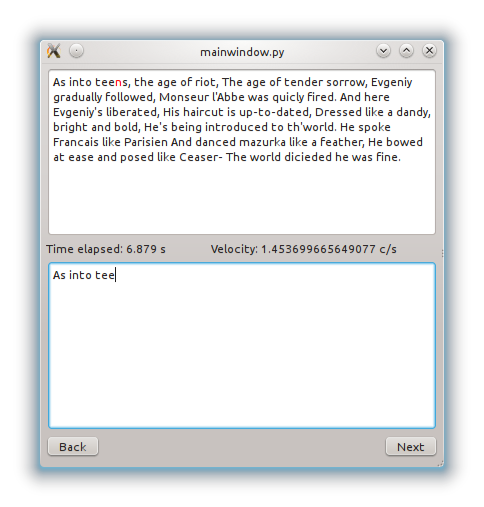
\includegraphics[scale=0.5]{images/trainer.png}
    \caption{Вид окна тренажера}
    \label{fig:trainer}
\end{figure}

Листинги кода всех виджетов приведены в приложении А.

\subsection{Работа с базой данных}
\label{sec:db}

Как уже неоднократно выше упоминалось, данное приложение в качестве базы данных использует SQLite 3-й версии.

Схема разработанной базы данных приведена на рисунке \ref{fig:db}

\begin{figure}[h!]
    \centering
    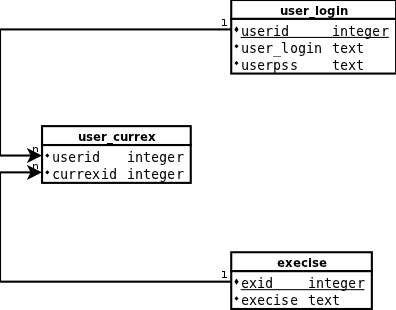
\includegraphics[scale=0.5]{images/db.png}
    \caption{Схема базы данных}
    \label{fig:db}
\end{figure}

Схема базы данных достаточно проста: хранению подлежит информация о текущем пользователе (логин и пароль), 
а также текст упражнений. Необходимо также ввести промежуточную таблицу, что обеспечивает решение проблемы 
связности, присущей всем sql-подобным базам данных.

Для взаимодействия с разработанной базой данных был создан специальный класс, который реализует концепцию DAO.
Также при проектировании данного класса был задействован паттерн Singleton. Методы класса предоставляют доступ
к информации, хранящейся в БД, тем самым производится отделение логики программы от используемых ею данных.

Код реализации приведен в листинге \ref{lst:dao}

\lstinputlisting[language=Python, caption=Реализация взаимодействия с базой данных, label=lst:dao]{src/mydao.py}

